\documentclass[border=2pt]{standalone}

\usepackage{tikz}
    \usetikzlibrary{math, calc}
\usepackage{siunitx}

\begin{document}
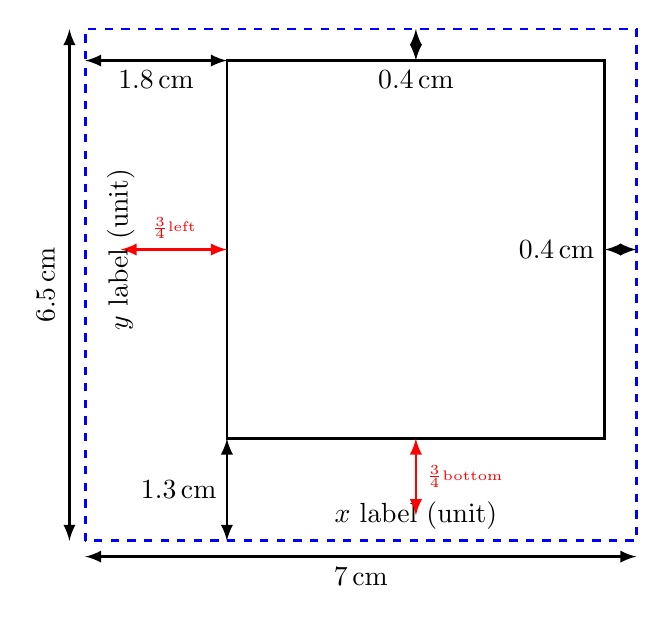
\begin{tikzpicture}[line width=1pt]
    \tikzmath{
        \figweight=7;
        \figheight=6.5;
        \axleft=1.8;
        \axright=0.4;
        \axbottom=1.3;
        \axtop=0.4;
        \axweight=\figweight-\axleft-\axright;
        \axheight=\figheight-\axbottom-\axtop;
    }

    \coordinate (O) at (0, 0);
    \draw [dashed, blue] (O) rectangle ++(\figweight, \figheight);
    \draw ($ (O) + (\axleft, \axbottom) $) rectangle ($ (O) + ({\figweight-\axright}, {\figheight-\axtop}) $);

    % x label
    \node at (\axleft+\axweight/2, \axbottom/4) {$ x~\mathrm{label}~\mathrm{(unit)}$};
    \draw [red, latex-latex] (\axleft/4, \axbottom+\axheight/2) -- (\axleft, \axbottom+\axheight/2) node [midway, above] {\tiny $ \frac{3}{4}\mathrm{left} $};

    % y label
    \node [rotate around={90:(0, 0)}] at (\axleft/4, \axbottom+\axheight/2) {$ y~\mathrm{label}~\mathrm{(unit)} $};
    \draw [red, latex-latex] (\axleft+\axweight/2, \axbottom/4) -- (\axleft+\axweight/2, \axbottom) node [midway, right] {\tiny $ \frac{3}{4}\mathrm{bottom} $};

    % figure size indicator
    \draw [latex-latex] ($ (O) + (-0.2, 0) $) -- ++(0, \figheight);
    \node [rotate around={90:(0, 0)}] at (-0.5, \figheight/2) {$ \qty{\figheight}{\centi\meter} $};
    \draw [latex-latex] ($ (O) + (0, -0.2) $) -- ++(\figweight, 0)
    node [below, midway] {$ \qty{\figweight}{\centi\meter} $};

    % axes size indicator
    % 左侧
    \draw [latex-latex] (0, \figheight-\axtop) -- (\axleft, \figheight-\axtop)
    node [below, midway] {$ \qty{\axleft}{\centi\meter} $};
    % 底部
    \draw [latex-latex] (\axleft, 0) -- (\axleft, \axbottom)
    node [left, midway] {$ \qty{\axbottom}{\centi\meter} $};
    % 顶部
    \draw [latex-latex] (\axleft+\axweight/2, \figheight) -- (\axleft+\axweight/2, \figheight-\axtop)
    node [below] {$ \qty{\axtop}{\centi\meter} $};
    % 右侧
    \draw [latex-latex] (\figweight, \axbottom+\axheight/2) -- (\figweight-\axright, \axbottom+\axheight/2)
    node [left] {$ \qty{\axright}{\centi\meter} $};
\end{tikzpicture}
\end{document}